% Dieser Text ist urheberrechtlich geschützt
% Er stellt einen Auszug eines von mir erstellten Referates dar
% und darf nicht gewerblich genutzt werden
% die private bzw. Studiums bezogen Nutzung ist frei
% Januar 2006
% Autor: Sascha Frank 
% Universität Freiburg 
% www.informatik.uni-freiburg.de/~frank/
% www.namsu.de/


\documentclass{beamer}
%%\usetheme{Warsaw-seahorse}
%\usepackage{german}
%\usepackage{ngerman}
\usepackage[utf8]{inputenc}
\usepackage[ngerman]{babel}
\usepackage{hyperref}

\usetheme{Warsaw}
%\usecolortheme{seahorse}
%\usefonttheme{serif}
\useinnertheme{rectangles}
%\usepackage{bookman}
\setbeamercovered{transparent}

%\setbeamertemplate{navigation symbols}{}
%\setbeamertemplate{footline}{}
%\setbeamertemplate{headline}{}


\usepackage{color} % used for comments
\usepackage{listings}%Quellcode

\usepackage{wrapfig}%floating elements

\definecolor{Navy}{rgb}{0,0,0.5}
\definecolor{Gray}{gray}{0.5}
\definecolor{dunkelgrau}{rgb}{0.8,0.8,0.8}
\definecolor{hellgrau}{rgb}{0.95,0.95,0.95}
\definecolor{hellgrau2}{rgb}{0.93,0.93,0.93}
\definecolor{red}{rgb}{1,0, 0.2}
\definecolor{green}{rgb}{0,1,0.2}

\lstset {
  language=xml,
  basicstyle={\footnotesize\ttfamily},
  numbers=none,
  aboveskip=5mm,
  belowskip=5mm,
  showstringspaces=false,
  columns=flexible,
  keywordstyle={\bfseries\color{green}},
  commentstyle={\color{Red}\textit},
  stringstyle={\color{red}},
  frame=single,
  breaklines=true,
  breakatwhitespace=true,
  tabsize=4,
  morekeywords={xmlns:rdf, xmlns:rdfs, rdf:about, rdf:resource}  % <-- adding custom keywords
}
\lstset {
  language=sparql,
  basicstyle={\footnotesize\ttfamily},
  numbers=left,
  aboveskip=5mm,
  belowskip=5mm,
  showstringspaces=false,
  columns=flexible,
  keywordstyle={\bfseries\color{green}},
  commentstyle={\color{hellgrau}\textit},
  stringstyle={\color{red}},
  frame=single,
  breaklines=true,
  breakatwhitespace=true,
  tabsize=4,
  morekeywords={PREFIX, select, SELECT, where, WHERE, Filter, filter, FILTER}  % <-- adding custom keywords
}

% Fußnoten korrigieren:
\makeatletter
 \renewcommand\@makefntext[1]{%
  \setlength{\hangindent}{2em}
  \noindent
  \hb@xt@\hangindent{%
     \hss\@textsuperscript{\normalfont\@thefnmark}\hspace{.1em}}#1}
\makeatother


\begin{document}

\title{Masterseminar}
\subtitle{Untersuchung und Optimierung verteilter geografischer Informationssysteme zur Verarbeitung agrartechnischer Kennzahlen} 
\author{Kurt Junghanns, B.Sc. \\(kjungha@htwk-leipzig.de)} 
\date{\today}
%\logo{\includegraphics[scale=0.08]{logo-SF}}
 
\begin{frame}
\titlepage
\end{frame}

\begin{frame}
\frametitle{Inhaltsverzeichnis}\tableofcontents
\end{frame}

\section{Einleitung}
\begin{frame}\frametitle{Einleitung}
\underline{Betreuer:}\\
M. Sc. Volkmar Herbst\\
Prof. Dr. rer. nat. Thomas Riechert\\
\vspace{\baselineskip}
\begin{wrapfigure}{r}{0.66\textwidth}\centering
    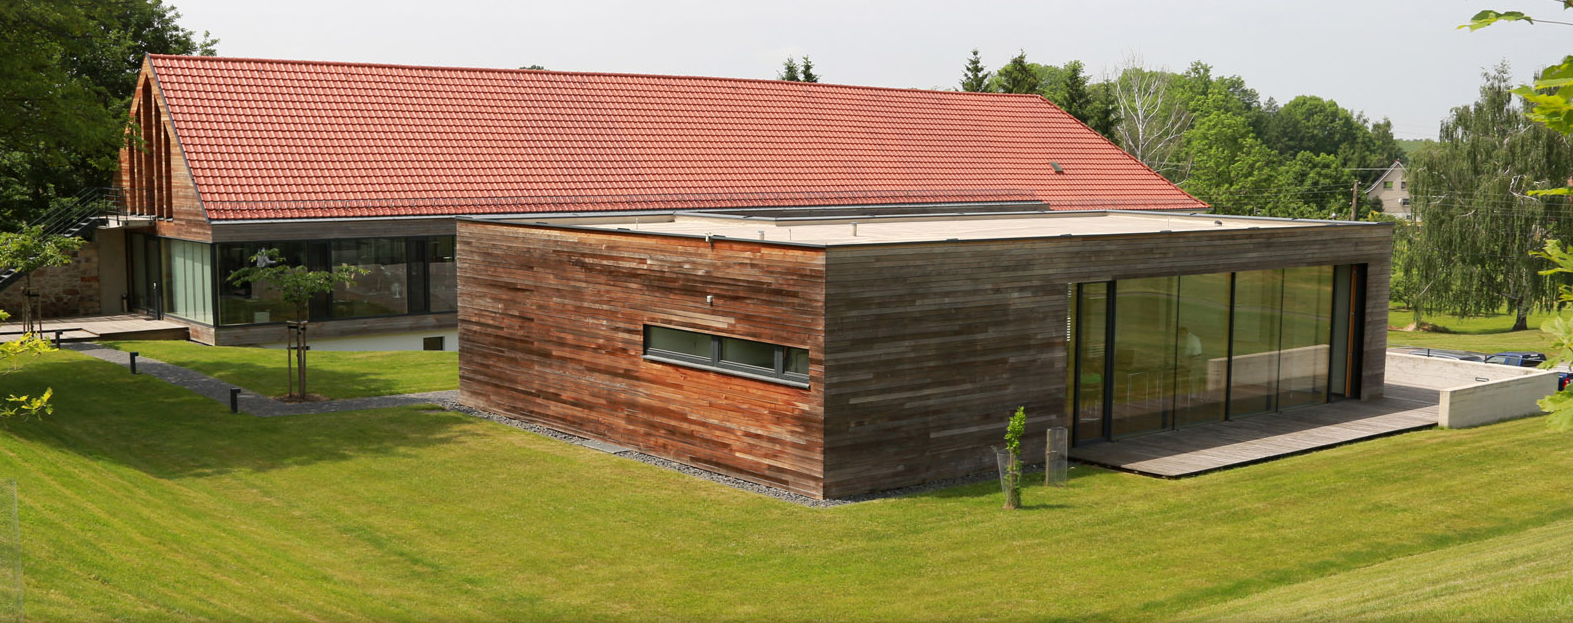
\includegraphics[scale=0.21]{Firma.png}
    %\caption{Image3.png}
\end{wrapfigure}
\underline{Unternehmen:}\\
Agri Con GmbH\\\url{http://agricon.de}\\
% Datenerfassung über Sensoren und Probenahmegräte 
% Technik (Elekktronik) und Erfahrungen
% Einsatzplanung von Maschinen, Betriebsmitteln und Arbeitszeit
% EInklang von Ertrags- und Qualitätsziele mit den wachsenden Umweltanforderungen
% Sensoren, GPS, Terminal, Telemetrie, Datenmanegement, Grunddüngung
\vspace{\baselineskip}
\underline{Abgabedatum:}\\
28.3.2015
\end{frame}

\section{Aufgabenstellung}
\begin{frame}\frametitle{Aufgabenstellung}
\textit{Untersuchung und Optimierung verteilter geografischer Informationssysteme zur Verarbeitung agrartechnischer Kennzahlen:}\\

% Informationssystem nach Kudraß:
% S. 32
% "Ein Informationssystem (IS) dient der rechnergestützten Erfassung, Speicherung, Verarbeitung, Pflege, Analyse, Verbreitung, Übertragung und Anzeige von Informationen. Es ist ein soziotechnisches System, das menschlische und maschinelle Komponenten (Teilsysteme) für die optimale Bereitstellung von Informationen und Kommunikation umfasst."
% geometrische und tplologische Eigenschaften werden berücksichtigt

\begin{enumerate} %GIS erklären
\item Untersuchung bestehender Frameworks für GIS anhand von Qualitätsmerkmalen
\item Auswahl eines Frameworks
\item Entwurf (Architektur, Konfiguration und Erweiterung)
\item Prototypische Implementierung %plus Bewertung
\end{enumerate}
\end{frame}

\section{Einordnung}
\begin{frame}\frametitle{Ziele für Agri Con} 
\begin{block}{Interesse von:}
%\underline{Interesse von:}\\
\begin{itemize}
\item Existierenden OpenSource Alternativen
\item NoSQL Eignung
\item Verringerung der Verarbeitungszeit für Daten
\end{itemize}
\end{block}

\begin{block}{Zur Anwendung für:}
%\underline{Zur Anwendung für:}\\
\begin{itemize}
\item Entlastung der Datenbank
\item Persistierung der originalen Daten
\item Verringerung der Verarbeitungszeit für Daten
\end{itemize}
\end{block}
\end{frame}

\section{Grundlagen}
\begin{frame}\frametitle{Arbeitsgrundlage} 
\begin{itemize}
\item Referenzsystem (PostGIS\footnote{GIS Erweiterung für PostgreSQL: \url{http://postgis.org}} und R\footnote{freie Programmiersprache für statistisches Rechnen}) %Ist Stand
\item Testdaten\footnote{Punkt-, Vektor- und Rasterdaten}
%Pflanzenbauliche Daten: Punktdaten; Basisdaten wie Feldgrenze: Vektordaten; Externe Satelliteninformationen und Multispektralanalysen: Rasterdaten

\item Anforderungen
\item Ausgabemodul (UMN MapServer)
\end{itemize}
\end{frame}

\begin{frame}\frametitle{Grundlegende Methoden} 
\begin{itemize}
\item Softwarequalität\footnote{Wallmüller, Ernest: Software-Qualitätsmanagement in der Praxis: Software-Qualität durch Führung und Verbesserung von Software-Prozessen. 2. Auflage. Hanser-Verl., 2001}
\item Softwaremetriken\footnote{Fenton, Norman E.; Pfleeger, Shari Lawrence: Software metrics: a rigorous and practical approach. PWS Publ. Comp., 1997}
\item Funktionstests\footnote{Ludewig, Jochen; Lichter, Horst: Software-Engineering: Grundlagen, Menschen, Prozesse, Techniken. dpunkt-Verl., 2007}
\item Leistungstests\footnote{Hansen, Olav: Leistungsanalyse paralleler Programme. Spektrum, 1995}
\item Nutzwertanalyse
%nicht Capability Maturity Model (Reifegradmodell) (kurz CMM), da es um Entwicklung/Verbesserung von Software geht
%nicht Control Objectives for Information and Related Technology (COBIT), da Unternehmen nicht in die Analyse einfließen soll
%Analytic Hierarchy Process (AHP) [auch nicht geeignet, da keine Teams und Zeitmanagement] zu detailiert, da maximal 1 System die notwendigen Anforderungen erfüllt und somit keine detailierte Abschätzung/Bewertung der systeme gegeben werden muss
%
%\item Guidelines der Systeme
\end{itemize}
\end{frame}

%\section{Eigentanteil}
% Vorhandene Systeme in diesem Anwendungsszenario vergleichen
% erweiterung der Syteme durch eigenen Code und andere Systeme
% 

\section{Anforderungen}
\begin{frame}\frametitle{Anforderungen}
Die prototypische Umsetzung ist Wunschkriterium.\\ %da Eignung der Systeme zu Beginn nicht bekannt

\vspace{\baselineskip}


Ziel ist bei Eignung von Systemen das mit der bestmöglichen Eignung zum Einsatz in der Firma darzustellen.
\end{frame}

\begin{frame}\frametitle{Qualitätskriterien}
\begin{itemize}
\item Funktionsumfang: parallele Verarbeitung, Gruppierungs-, Filter-, Verschneidungs- sowie Overlayfunktionen und Geostatistik
\item Interoperabilität: Schnittstellen für PostgreSQL und UMN MapServer
\item Fehlertoleranz: Unabhängigkeit der Verarbeitungsprozesse
\item Dokumentation: Vorhandene und aktuelle Dokumentation der Installation, Verwendung und Wartung
\item Zeitverhalten: Verarbeitungszeiten unter denen des Ist-Standes\footnote{Abhängig von Art der Berechnung und Menge der Daten}
\end{itemize}
\end{frame}

\section{Lösungsansatz}
%modellieren der Aufgabe, den Kontext und die Ergebnisse


\begin{frame}\frametitle{Ansätze zur Lösung}
\begin{block}{Softwareauswahl:}
%\underline{Softwareauswahl:}\\
Bewertung von Software durch Nutzwertanalyse mit Hilfe von Qualitätsmerkmalen und -kriterien.\\
\end{block}
\vspace{\baselineskip}
\begin{block}{Bewertung:}
%\underline{Bewertung:}\\
Softwaremetriken mit Leistungs- und Funktionstests.
\end{block}
\end{frame}
%aus Studium:
% Messung des Speedup aus MessagePassing
% 

\section{Projektstand}
\begin{frame}\frametitle{Planung}
%Gantt
\begin{figure}[htb]
  \begin{center}
    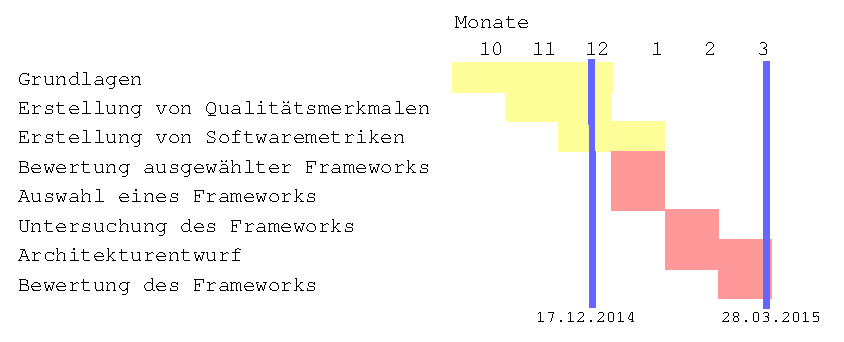
\includegraphics[width=1\hsize]{Plan_cropped.pdf}
  \end{center}
  %\caption[a]{}
\end{figure}
\end{frame}


\begin{frame}\frametitle{Offene Arbeiten}
\begin{itemize}
\item Softwaremetriken spezifizieren
\item Systeme auswählen
\item ausgewählte Systeme mit Metriken bewerten
\item Prototyp entwerfen
\item Werkzeugauswahl
\item Prototyp bewerten
\end{itemize}
\end{frame}

\begin{frame}\frametitle{Diskussion}
%3 Fragen formulieren
\begin{block}{}
Existiert eine Handlungsempfehlung zur Auswahl von Werkzeugen zur Durchführung von Funktions- und Leistungstests?
\end{block}
\vspace{\baselineskip}
\begin{block}{}
Existieren wissenschaftliche Dokumente zu Nutzwertanalyse bei der Softwarebeschaffung?
\end{block}
%\vspace{\baselineskip}


\end{frame}

\end{document}
